\documentclass[
    11pt,
    spanish,
    a4paper
]{article}
\usepackage[utf8]{inputenc}
\usepackage[spanish]{babel}
\usepackage{authoraftertitle}
\usepackage{booktabs}
\usepackage{caption}
\usepackage{float}
\usepackage{graphicx}
\usepackage{listings}
\usepackage{verbatim}
\usepackage{amsmath}
\usepackage{amsfonts}

\def\doctype{Trabajo práctico}
\title{Markov y PFD}
\author{Gonzalo Nahuel Vaca}

\begin{document}

\makeatletter
\begin{titlepage}
	\begin{center}
		\vspace*{1cm}

		\Huge
		\textbf{\doctype}
		\vspace{0.5cm}

		\LARGE
		\@title
		\vspace{0.5cm}

		\textbf{Introducción a los sistemas críticos}

		\vspace{1.5cm}

		\textbf{\@author}

		\vspace{1.5cm}

		
\includegraphics[width=0.8\textwidth]{img/logoFIUBA.pdf}

		\vfill
		Maestría en Sistemas Embebidos\\
		Universidad de Buenos Aires\\
		Argentina\\
		\today
	\end{center}
\end{titlepage}
\makeatother
\newpage

\section{Enunciado}

Considere una estructura en serie de dos componentes. Cuando uno de los componentes falla, el otro
componente queda inmediatamente fuera de servicio hasta que el componente defectuoso se repara.
Después de que un componente se retira del funcionamiento, no está expuesto a ningún estrés.

NOTA: El mismo modelo es discutido por Barlow y Proschan (1975, pp. 194-201) en un contexto más general que no
supone tasas constantes de fallas y reparaciones.

\begin{center}
	\begin{tabular}{c c c}
		\hline
		Estados & Componente 1       & Componente 2       \\
		\hline
		2       & Funcionando        & Funcionando        \\
		1       & Fuera de operación & Funcionando        \\
		0       & Funcionando        & Fuera de operación \\
		\hline
	\end{tabular}
\end{center}

\begin{itemize}
	\item Realizar diagrama de transición de estados.
	\item Escribir la ecuación matricial de proceso de Markov para estados estacionarios.
	\item Siendo $ \lambda=10^{-3} $ y el tiempo de inactividad promedio requerido para la reparación del componente $ i $ es 8 horas, $ MDT_i $. Calcular:
	      \begin{enumerate}
		      \item Probabilidad de que el sistema esté en cada uno de los estados, $ P_j $.
		      \item Indisponibilidad del sistema $ \bar{A_s} $.
		      \item Duración media de que el sistema permanezca en cada uno de los estados, $ \theta_j $ .
		      \item Frecuencia de falla del sistema, $ \omega_F $
		      \item Tiempo medio entre fallas del sistema, $ MTBF_s $.
		      \item Tiempo medio de falla del sistema, $ MTTF $.
	      \end{enumerate}
	\item Analice otro diagrama de transición de estados si los dos componentes estuvieran en paralelo.
\end{itemize}

Nota: En cada uno de los puntos, escribir la fórmula utilizada.

\section{Resolución}

\subsection{Realizar diagrama de transición de estados.}

En la figura \ref{fig:diagrama_estados} se puede observar el diagrama de estados. Se realizó en \emph{Plantuml}.
Como los componentes están en serie y al fallar uno el otro sale de servicio, entonces solo el estado '2' supone que el sistema se encuentra en funcionamiento.

\begin{figure}[htbp]
	\centering
	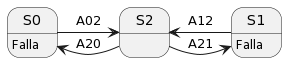
\includegraphics[width=0.5\textwidth]{img/diagrama_estados.png}
	\caption{Diagrama de estados.}
	\label{fig:diagrama_estados}
\end{figure}

Donde:

$ a_{21} = \lambda_1 $; Transición de '2' a '1': tasa de falla del componente 1

$ a_{12} = \mu_1 $; Transición de '1' a '2': tasa de reparación del componente 1

$ a_{20} = \lambda_2$; Transición de '2' a '0': tasa de falla del componente 1

$ a_{02} = \mu_2$; Transición de '0' a '2': tasa de reparación del componente 1

Cuando un componente falla el otro se retira de servicio.
En esta condición, el componente retirado no sufre desgastes y por lo tanto $ a_{01} = a_{10} = 0 $.
Esto quiere decir que el sobreviviente no puede fallar.

\subsection{Escribir la ecuación matricial de proceso de Markov para estados estacionarios.}

Según las diapositivas 15 y 16 del apunte 'Teoría de Confiabilidad', las ecuaciones de estados se pueden definir de la siguiente manera:

$$ \dot{\mathbb{P}(t)} = \mathbb{P}(t) . \mathbb{A} $$

Donde:
\begin{itemize}
	\item $ \mathbb{P}(t) $: matriz de estados cuyas entrada es la probabilidad de transición del proceso Markov.
	\item $ \mathbb{A} $: matriz de tasas de transición.
\end{itemize}

Alternativamente (según diapositiva 18) se puede expresar de la siguiente manera:

\begin{equation}
	[\dot{P_0(t)},\dot{P_1(t)},\dot{P_2(t)}] =
	\begin{pmatrix}
		P_{00}(t) & P_{01}(t) & P_{02}(t) \\
		P_{10}(t) & P_{11}(t) & P_{12}(t) \\
		P_{20}(t) & P_{21}(t) & P_{22}(t)
	\end{pmatrix} *
	\begin{pmatrix}
		a_{00} & a_{01} & a_{02} \\
		a_{10} & a_{11} & a_{12} \\
		a_{20} & a_{21} & a_{22}
	\end{pmatrix}
\end{equation}

En sistemas estacionarios, según diapositiva 13 deben satisfacer:

\begin{equation}
	[0,0,0] = [P_0(t),P_1(t),P_2(t)] *
	\begin{pmatrix}
		-\mu_2    & 0         & \mu_2                   \\
		0         & -\mu_1    & \mu_1                   \\
		\lambda_2 & \lambda_1 & (\lambda_1 + \lambda_2)
	\end{pmatrix}
\end{equation}

\subsection{Siendo $ \lambda=10^{-3} $ y el tiempo de inactividad promedio requerido para la reparación del componente $ i $ es 8 horas, $ MDT_i $. Calcular:}


\subsubsection{Probabilidad de que el sistema esté en cada uno de los estados, $ P_j $.}

Lo primero que se toma en cuenta es que el dato $ \lambda=10^{-3} $ aplica para los dos componentes en serie.
Esto significa que:

$$ \lambda=\lambda_1=\lambda_2=10^{-3} $$

Además, como los componentes están en serie:

$$ MDT_i = \frac{1}{\mu_i} $$

Como el tiempo de inactividad promedio requerido para la reparación del componente $ i $ es de 8 horas:

$$ \mu_1 = \mu_2 = 0.125 $$

A partir del desarrollo del punto anterior:

$ P_0 + P_1 + P_2 = 1 $; Dado el espacio muestral de tres estados posibles, la probabilidad de encontrase en uno de esos estados es 1.

Además, del producto matricial se puede obtener que:

$$ -\mu_2 * P_0 + \lambda_2 * P_2 = 0 $$
$$ -\mu_1 * P_1  + \lambda_1 * P_2 = 0 $$
$$  \mu_2 * P_0 + \mu_1 * P_1 - (\lambda_1 + \lambda_2) * P_2 = 0 $$

Se debe recordar que $ \lambda=\lambda_1=\lambda_2=10^{-3} $ y que $ \mu = \mu_1 = \mu_2 = 0.125 $.
Con esto en mente las ecuaciones quedan de la siguiente manera:

$$ -\mu * P_0 + \lambda * P_2 = 0 $$
$$ -\mu * P_1 + \lambda * P_2 = 0 $$
$$  \mu * P_0 + \mu * P_1   - 2 * \lambda * P_2 = 0 $$

Finalmente:

$$ P_0 = 0.069 $$
$$ P_1 = 0.069 $$
$$ P_2 = 0.862 $$

Nota: este razonamiento es válido solo porque los componentes se encuentran en serie.

\subsubsection{Indisponibilidad del sistema $ \bar{A_s} $.}

A partir del ejemplo 8.6 de las diapositivas se puede definir la indisponibilidad de dos componentes en serie como:


$$ A_s = \frac{\mu_1*\mu_2}{\lambda_1*\mu_2+\lambda_2*\mu_1+\mu_1*\mu_2}$$
$$ A_s = \frac{\mu *\mu}{\lambda*\mu+\lambda*\mu+\mu*\mu}$$
$$ A_s = \frac{(0.125)^2}{10^{-3} * 0.125 +0.125 * 10^{-3}+(0.125)^2}$$
$$ A_s = \frac{0,015625}{0,000125+0,000125+0,015625}$$
$$ A_s = \frac{0,015625}{0,015875}$$
$$ A_s = 0,984251969$$
$$ \bar{A_s} = 1 - A_s = 0,015748031 $$


\subsubsection{Duración media de que el sistema permanezca en cada uno de los estados, $ \theta_j $ .}

A partir de la siguiente definición:

$$ \theta_j = \frac{1}{\alpha_j} = \frac{1}{\sum_{k=0, k \neq j}^{r} a_{kj}} $$

\subsubsection{Frecuencia de falla del sistema, $ \omega_F $}
\subsubsection{Tiempo medio entre fallas del sistema, $ MTBF_s $.}
\subsubsection{Tiempo medio de falla del sistema, $ MTTF $.}


\subsection{Analice otro diagrama de transición de estados si los dos componentes estuvieran en paralelo.}

\begin{figure}[htbp]
	\centering
	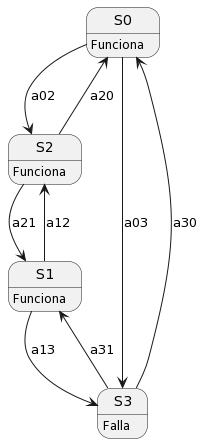
\includegraphics[width=0.3\textwidth]{img/diagrama_estados_2.png}
	\caption{Diagrama ejercicio 4.}
	\label{fig:diagrama_estados_2}
\end{figure}

$ a_{21} = \lambda_1 $, Tasa de falla del componente 1

$ a_{12} = \mu_1 $, Tasa de reparación del componente 1

$ a_{20} = \lambda_2 $, Tasa de falla del componente 2

$ a_{02} = \mu_2 $, Tasa de reparación del componente 2

$ a_{13} = \lambda_2 $, Tasa de falla del componente 2

$ a_{31} = \mu_2 $, Tasa de reparación del componente 2

$ a_{03} = \lambda_1 $, Tasa de falla del componente 1

$ a_{30} = \mu_1 $, Tasa de reparación del componente 1

\end{document}